\chapter{Laser Interferometer Space Antenna}\label{chap:lisa}
[REFERENCES: \cite{babak2021lisasensitivitysnrcalculations}, \cite{PhysRevD.95.103012}]\\
The LISA project is a space-based gravitational wave detector (\cite{colpi2024lisadefinitionstudyreport}) that is currently under development led by the European Space Agency (ESA) in collaboration with NASA and the LISA consortium after being adopted in early 2024\footnote{\url{https://www.esa.int/Science_Exploration/Space_Science/LISA/Capturing_the_ripples_of_spacetime_LISA_gets_go-ahead}} and constructions will start in early 2025. Not only will LISA be the first space-based gravitational wave detector, but it will also be the first detector to observe gravitational waves in the millihertz frequency range. This frequency range is inaccessible to ground-based detectors like LIGO and Virgo due to the seismic noise that dominates at these low frequencies and the limitations on the armlengths of the detectors. For this reason LISA will open the door to a new era in gravitational wave astronomy in terms of precision but also in terms of the type of events that we can observe, one of them being the inspiral of a compact object around a supermassive black hole, i.e. extreme mass ratio inspirals (EMRIs). In this chapter we will discuss the LISA detector, its response to gravitational waves and the data analysis techniques that are used to extract the signals from the noise.

\section{The LISA mission}
The LISA mission consists of three spacecrafts that are arranged in an almost equilateral triangle with an armlength of $2.5 \times 10^6\unit{km}$ and that are following the Earth in its orbit around the Sun. The spacecrafts will exchange coherent laser beams to function as a set of Michelson interferometers.

\section{Measurements with LISA}
Before we can start doing data analysis with LISA measurements we need to understand how the detector works, what a given signal looks like in the detector frame and what is the response of the detector to the gravitational wave signal. This section is meant to give an overview of what we will discuss in the following sections. The gravitation wave signal that is produced by an EMRI event or more in our case the template of an EMRI event is at first is theoretically predicted in the source frame and in the framework of general relativity using different perturbative approximations mentioned in \fullref{chap:emris}. This will correspond to $h(t) = h_+(t) + h_\times(t)$ where $h_+(t)$ and $h_\times(t)$ are the two polarizations of the gravitational wave signal as we have found in \fullref{chap:gravitational_waves}. The signal then propagates through spacetime until it hits the detector. Theoretically, we can retrace this in two steps, the first being to transform the signal into the SSB frame and then transform it into the rotating detector frame of LISA. This is characterized by the \emph{antenna pattern functions} of the detector. The antenna patter functions carry the information how the interferometer is aligned with respect to the polarizations of the gravitational wave in the transverse-traceless gauge for example. At this point we now have the signal right before it enters the detector and the further consideration will then produce the \emph{response} of the detector to given signal. This will be strongly restricted by the sensitivity of the detector.  As one continues to take more and more details of the motion of the detector and the detector itself into account, one finally ends up with what is called Time Delay interferometry (TDI) but more on that later.

\section{LISA sensitivity}
In \fullref{sec:parameter-estimation} we derived how we can compute the optimal SNR of a given signal (or EMRI waveform template) in the presence of noise of the detector characterized by noise spectral density \fullref{eq:noise-spectral-density-definition}. This reduced to the scalar product given in \fullref{eq:scalar-product}
\begin{equation}
    \left(\frac{S}{N}\right)^2 = 4 \Re \int_{0}^{\infty} \dd{f} \frac{\abs{\tilde{h}(f)}^2}{\nsd}.
\end{equation}
So if we want to perform this calculation for LISA we need to know the noise spectral density $\nsd$ of the detector. In the latest study report of LISA \cite{colpi2024lisadefinitionstudyreport} the noise spectral density (see \fullref{fig:lisa-sensitivity}) is given as
\begin{equation}
    \nsd(f) = \frac{T_\text{acc}(f)S_\text{acc}(f) + T_\text{disp}(f) S_\text{disp}(f)}{R_\text{GW}(f)},
\end{equation}
where $T_\text{acc}(f)$ and $T_\text{disp}(f)$ are the transfer functions of the acceleration and displacement noise respectively, $S_\text{acc}(f)$ and $S_\text{disp}(f)$ are the acceleration and displacement noise spectral densities and $R_\text{GW}(f)$ is the response function of the detector to the gravitational wave signal. The transfer functions take into account what observables we are measuring with the detector. For us this will be the TDI channels $A,E,T$. But first let us discuss the noises that are considered in the noise spectral density. First, we have the \emph{acceleration noise} which is due to all sorts of forces that accelerate the test masses of the detector and is given in \cite{babak2021lisasensitivitysnrcalculations} in units of relative frequency
\begin{equation}
    \sqrt{S_\text{acc}(f)} = \frac{3 \times 10^{-15}}{(2 \pi f c )^2} \left(1 + \left(\frac{0.4\unit{mHz}}{f}\right)^2\right)\left(1 + \left(\frac{f}{8\unit{mHz}}\right)^4\right)\unitfrac{1}{\sqrt{Hz}}.
\end{equation}
Secondly, we have the \emph{displacement noise} which is dominated by the photon shot noise, i.e. by the time that the laser signal has traveled from one detector to the other the wavefront spreads out and becomes very weak once it hits the other detector. So weak in fact that the photon shot noise comes into play. The displacement noise is given in \cite{babak2021lisasensitivitysnrcalculations} by
\begin{equation}
    \sqrt{S_\text{disp}(f)} = 15 \times 10^{-12}\frac{2 \pi f }{c} \left(1 + \left(\frac{2\unit{mHz}}{f}\right)^4\right)\unitfrac{1}{\sqrt{Hz}}.
\end{equation}
This means now we are left with the response function of the detector to the gravitational wave signal and the transfer functions for the TDI channels $A,E,T$.

\begin{figure}
    \centering
    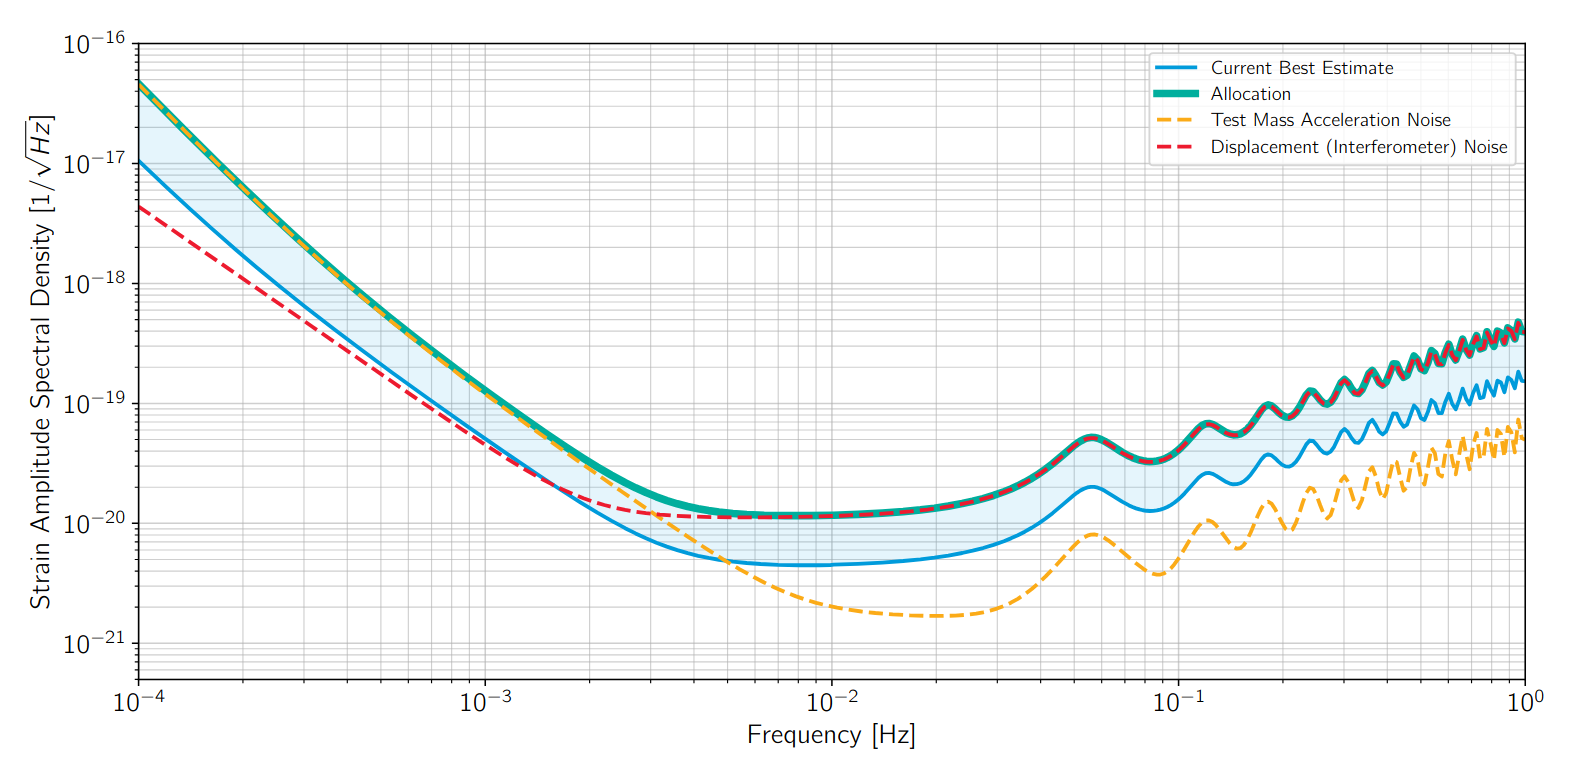
\includegraphics[width=0.8\textwidth]{LISA_sensitivity_strain.png}
    \caption[LISA spectral strain sensitivity]{The spectral strain sensitivity of LISA, which is $\sqrt{S_n(f)}$. The figure is taken from \cite{colpi2024lisadefinitionstudyreport}.}
    \label{fig:lisa-sensitivity}
\end{figure}

\subsection{Time delay interferometry}
For an introduction to TDI the reader is referred to \cite{Tinto_2021} or a rather recent in detail discussion of TDI in \cite{heisenberg2023lisadynamicscontrol}. Here we will try to summarize the idea of TDI and introduce the expressions that we are using in the data analysis.\\
For precise measurements with LISA it is crucial to suppress the laser noise that is present in the detector, which can occur from frequency variations of the electromagnetic signal, relative motions of the detectors (spacecrafts) and of course also from passing gravitational waves. The former of those, is the signal we want to measure amongst the noise. For a single Michelson interferometer with equal arm lengths the laser noise can be removed when the laser recombines at the detector. This however becomes a problem, if the arm lengths vary over time and thus the armlengths or no longer equal which leads to a phase difference and therefore a delayed fluctuations in the laser. To address this problem, the Time Delay Interferometry (TDI) was developed. This means the time-varying Doppler data needs to be recorded and then used to post-process the data. Let us consider the case for one Michelson interferometer with unequal arm lengths $L_1, L_2$ and let $C(t)$ be the fluctuations in the laser frequency. We will receive two Doppler data, one for each arm $y_1(t)$ and $y_2(t)$ (see \cite[Figure 1, Figure 2]{Tinto_2021} for further explanation). We will neglect any other noise source but think of a gravitational wave signal $h_1(t), h_2(t)$ that enters the signal. The Doppler measurements that we receive are then
\begin{equation}
    \begin{split}
        y_1(t) &= C(t - 2L_1) - C(t) + h_1(t),\\
        y_2(t) &= C(t - 2L_2) - C(t) + h_2(t),
    \end{split}
\end{equation}
and their difference is given by
\begin{equation}
    \begin{split}
        y_1(t) - y_2(t) &= C(t - 2L_1) - C(t) + h_1(t) - C(t - 2L_2) + C(t) - h_2(t)\\
        &= C(t - 2L_1) - C(t - 2L_2) + h_1(t) - h_2(t).
    \end{split}
\end{equation}
if we now also look at the time-delayed difference of the Doppler data, where we delay $y_1$ by $2L_2$ and $y_2$ by $2L_1$ we get
\begin{equation}
    \begin{split}
        y_1(t - 2L_2) - y_2(t - 2L_1) = C(t - 2L_1) - C(t - 2L_2) + h_1(t - 2L_2) - h_2(t - 2L_1).
    \end{split}
\end{equation}
This allows us to define a new observable that is free of the laser noise
\begin{equation}
    \boxed{X = \left[ y_1(t) + y_2(t - 2L_1) \right] - \left[y_2(t) +  y_1(t - 2L_2)\right].}
\end{equation}
This is a very simplified example of time delay interferometry. But what it boils down to is that we can construct new observables that are free of the laser noise such as the $X,Y,Z$ or $A,E,T$ channels. In our case we will use the $A,E,T$ channels because they are constructed such that $A,E$ carry the signal of the gravitational wave polarizations and $T$ is a so called \emph{null} or \emph{noise} channel. Further $A,E$ are orthogonal w.r.t to the scalar product \fullref{eq:scalar-product}, so we can just take the sum of both signals. For the detailed construction and the resulting noise spectral densities of the TDI channels we refer to \cite{Hartwig_2023}. As argued above the $T$ channel will not carry any signal, so we will neglect it. For the channels $A,E$ we have the following noise spectral density

\begin{equation}
    \boxed{
        \begin{aligned}
            \nsd^{(A,E)} & (f) =                                                                                                                                                                           \\
                         & 8 \sin^2\left(2\pi f L\right) \left \{ S_\text{disp}(f) \left[ \cos(2 \pi f L) + 2 \right] + 2\left[ 3 + 2\cos(2 \pi f L ) + \cos(4 \pi f L) \right] S_\text{acc}(f) \right \},
        \end{aligned}
    }
\end{equation}
where $L = 2.5 \times 10^6\unit{km}$ is the armlength of the detector and we went back to setting the arm lengths equal for the simulation we are considering here as we are not simulating the fluctuations in the detector arms. This means we can now compute the optimal SNR of a given signal in the presence of noise of the detector
\begin{equation}
    \label{eq:optimal-snr-lisa}
    \left(\frac{S}{N}\right)^2 = 4 \Re \int_{f_min}^{f_max} \dd{f} \frac{\abs{\tilde{A}(f)}^2 + \abs{\tilde{E}(f)}}{\nsd^{(A,E)}(f)},
\end{equation}
where $\tilde{A}(f), \tilde{E}(f)$ are the Fourier transforms of the $A,E$ channels that we will get from the results of \emph{fastlisaresponse} of the signal and $\nsd^{(A,E)}(f)$ is the noise spectral density of the $A,E$ channels. The limits of the integral are given by the bandwidth that LISA is sensitive to, which is chosen to $f_\text{min} = 10^{-5}, f_\text{max} = 1$.

    [TODO: add plots for noises and final psd]